% figures of the spectras

% figure Spectra_Al.png
\begin{figure}
    \centering
    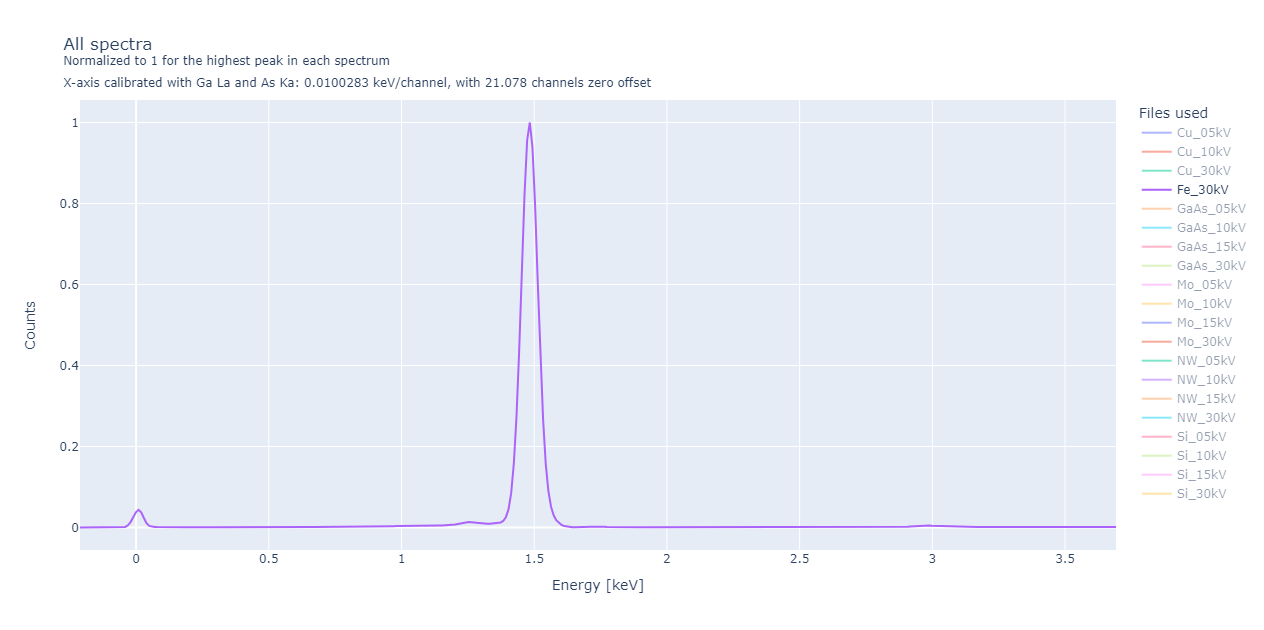
\includegraphics[width=0.70\textwidth]{figures/Spectra_Al.png}
    \caption{
        The spectra of the Al sample part.
        This was expected to be Fe, thus the label is wrong.
        The peak at 1.48 keV is the Al K$\alpha$ peak.
    }
    \label{fig:results:Spectra_Al}
\end{figure}

% figure Spectra_Cu.png
\begin{figure}
    \centering
    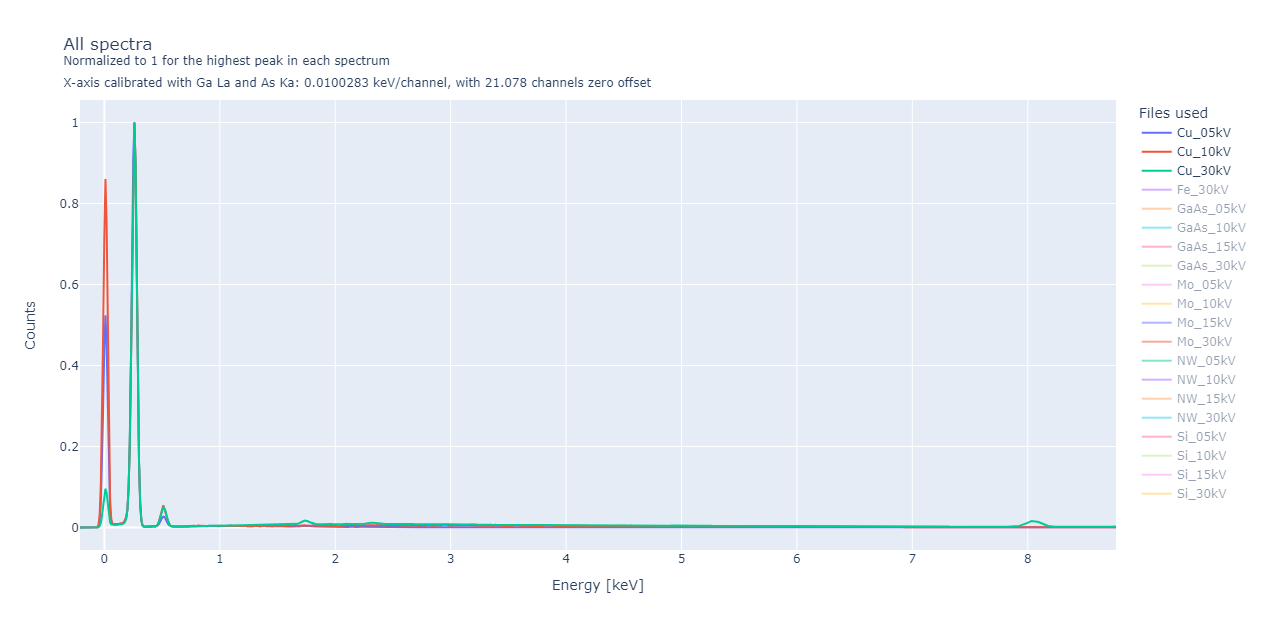
\includegraphics[width=0.70\textwidth]{figures/Spectra_Cu.png}
    \label{fig:Spectra_Cu}
    \caption{
        The spectra of the Cu sample part.
        The Cu sample was Cu-tape from the lab, but the Cu K$\beta$ peak is only barely visible at the 30 kV spectrum.
        The highest peak in all three spectra is at 0.260 keV, which is the C K$\alpha$ peak, slightly off from the expected 0.277 keV.
    }
\end{figure}

% figure Spectra_GaAs.png
\begin{figure}
    \centering
    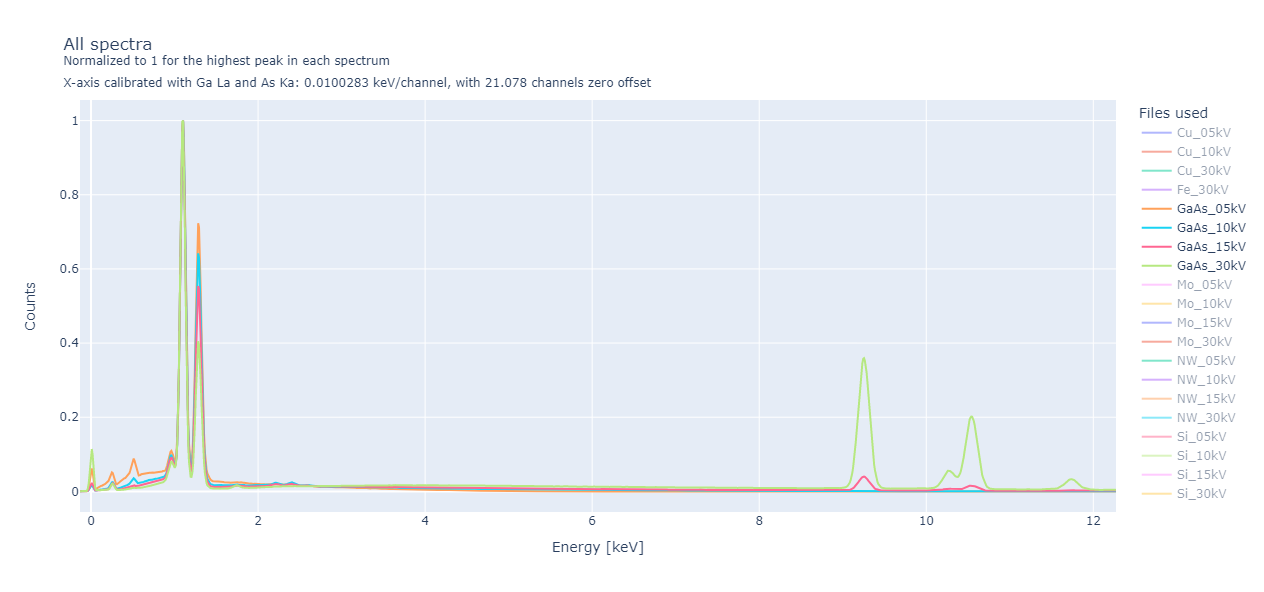
\includegraphics[width=0.70\textwidth]{figures/Spectra_GaAs.png}
    \label{fig:Spectra_GaAs}
    \caption{
        The spectra of the GaAs sample part.
        Both the K-peaks and the L-peaks of Ga and As are visible.
        There is a peak at 0.511 keV, which is the O K$\alpha$ peak.
        There is a peak at 0.260 keV, which is the C K$\alpha$ peak.
    }
\end{figure}

% figure Spectra_Mo.png
\begin{figure}
    \centering
    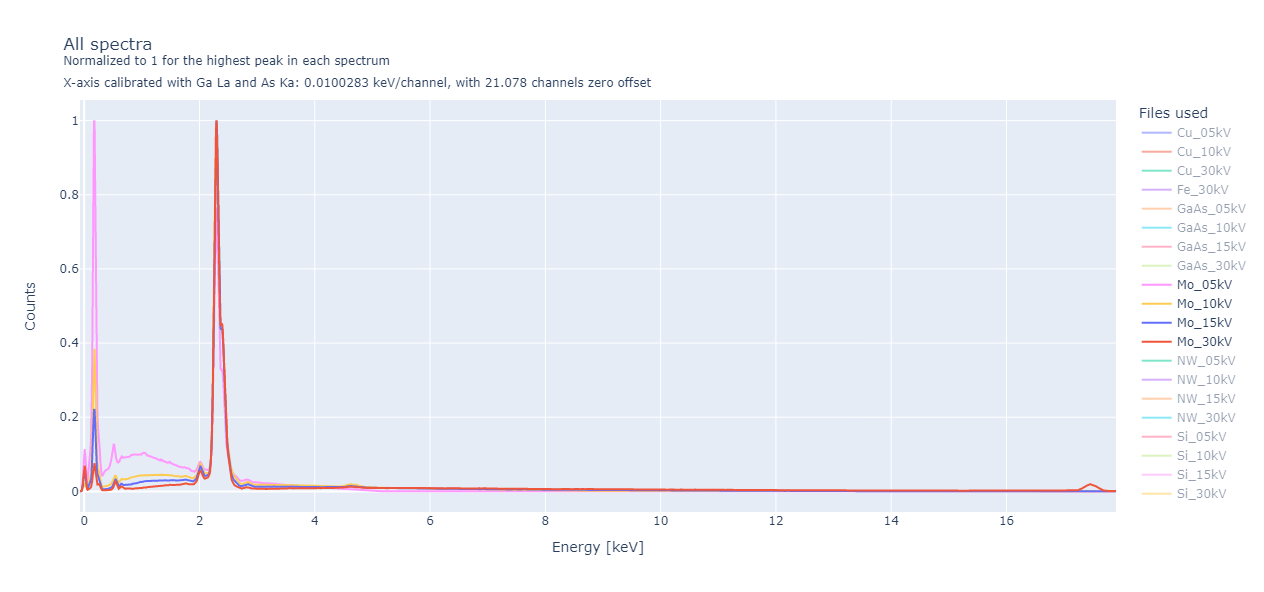
\includegraphics[width=0.70\textwidth]{figures/Spectra_Mo.png}
    \label{fig:Spectra_Mo}
    \caption{
        The spectra of the Mo sample part.
        The Mo K$\alpha$ peak at 17.47 keV is barely visible at the 30 kV spectrum, and has a high noise level.
        The high dobble peak is Mo L$\alpha$ at 2.29 keV and Mo L$\beta$ at 2.39 keV.
    }
\end{figure}

% figure Spectra_NW.png
\begin{figure}
    \centering
    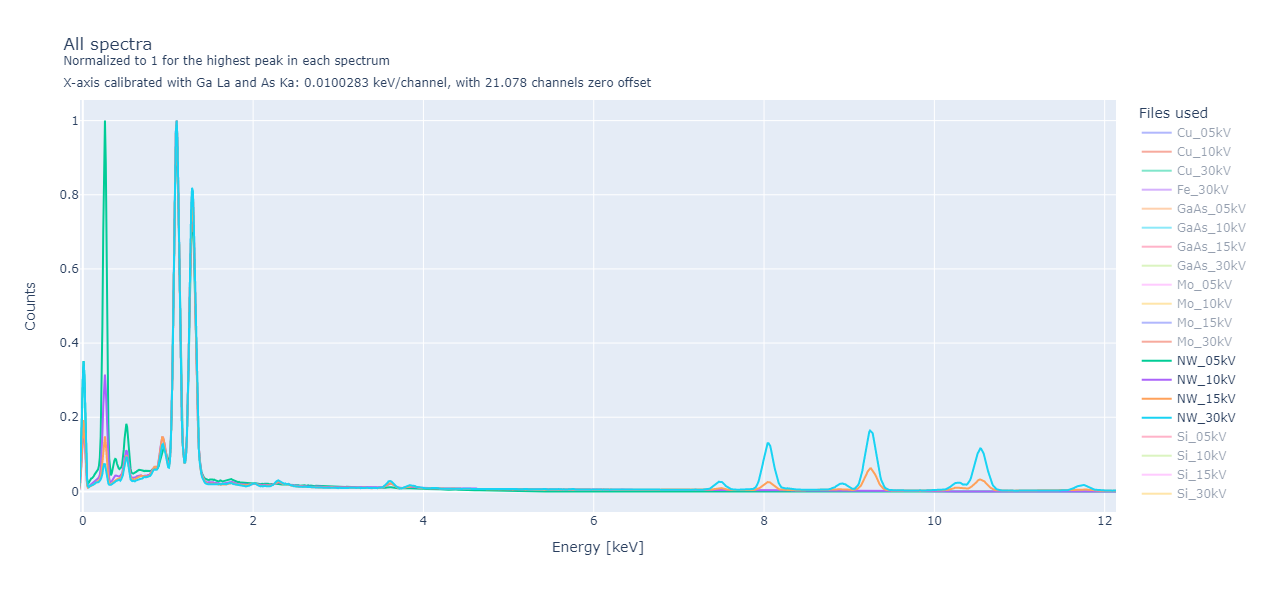
\includegraphics[width=0.70\textwidth]{figures/Spectra_NW.png}
    \label{fig:Spectra_NW}
    \caption{
        The spectra of the nanowire sample part.
        This spectrum have the most peaks, and contains Ga, As, Cu, Sb (? at 3.6 keV), Mo, C, and O.
    }
\end{figure}

% figure Spectra_Si.png
\begin{figure}
    \centering
    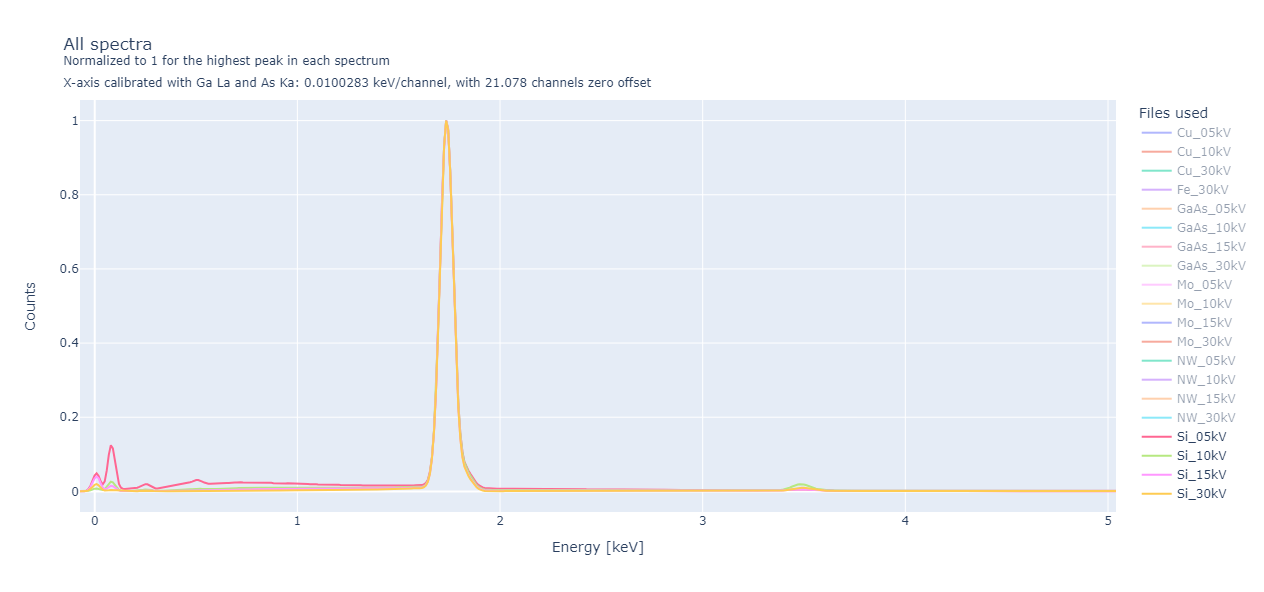
\includegraphics[width=0.70\textwidth]{figures/Spectra_Si.png}
    \label{fig:Spectra_Si}
    \caption{
        The spectra of the pure Si wafer sample part.
        All four spectra have one large peak at 1.73 keV, which is the Si K$\alpha$ peak.
        The four spectra also have a small peak at 3.48 keV, which is not identified.
    }
\end{figure}